\documentclass[twoside]{article} 
\usepackage[accepted]{aistats2017}

%%%%%%%%% User added packages %%%%%%%%%%%%%%
\usepackage{caption}
\RequirePackage{graphicx}
\usepackage{subcaption}
%\newcommand{\bth}{\bm{\theta}}
\newcommand{\la}{\lambda}
\newcommand{\bl}{\bm{\lambda}}
%\newcommand{\bxi}{\bm{\xi}}
\newcommand{\bsee}{\bm{\Sigma_e}}
\newcommand{\bo}{\bm{\Omega}}
\newcommand{\bD}{\bm{\Delta}}
%\newcommand{\bse}{\bm{\Sigma_e}^{-1}}
\newcommand{\bT}{\bm{t}}
%\newcommand{\bh}{\bm{H}}
\newcommand{\bc}{\bm{C}}
%\newcommand{\bd}{\bm{D}}
\newcommand{\bww}{\bm{W}}
%\newcommand{\ba}{\bm{A}}
\newcommand{\bbb}{\bm{B}}
\newcommand{\bg}{\bm{G}}
\newcommand{\bmy}{\bm{y}}
%\newcommand{\bys}{\bm{y^*}}
\newcommand{\bdd}{\bm{\delta}}
\newcommand{\bdh}{\hat{\bm{\delta}}}
%\newcommand{\byst}{\bm{y^{*T}}}

\newcommand{\thatb}{\hat{\bm{\theta}}^B}
\newcommand{\thatt}{\hat{\bm{\theta}}}
\newcommand{\thattt}{\hat{\bm{\theta_2}}}
\newcommand{\thp}{\hat{\bm{\theta}}^p}
\newcommand{\thg}{\hat{\bm{\theta}}^g}
\newcommand{\thbm}{\hat{\bm{\theta}}^{BM}}

\newcommand{\bty}{\tilde{\bm{\theta}}_{y,t}}
\newcommand{\su}{{\sigma_u^2}}
\newcommand{\thh}{{\theta}}
\newcommand{\bgam}{\bm{\gamma}}
\newcommand{\bth}{\bm{\theta}}
\newcommand{\bxi}{\bm{x}_i}
\newcommand{\bse}{\bm{\Sigma_e}^{-1}}
\newcommand{\bh}{\bm{H}}
\newcommand{\bd}{\bm{D}}
%\newcommand{\ba}{\bm{A}}
\newcommand{\bb}{\bm{\beta}}
% y\newcommand{\bxi}{\bm{x}_i}
\newcommand{\bys}{\bm{y^*}}
\newcommand{\byst}{\bm{y^{*T}}}
\newcommand{\V}       {\text{Var}}
\newcommand{\de}       {\mbox{$\delta_i$}}
\newcommand{\tij}       {\mbox{$\theta_{ij}$}}
\newcommand{\htijb}       {\mbox{$\hat{\theta}_{ij}^B$}}

\newcommand{\thbariw}     {\mbox{$\bar{\hat{\theta}}_{iw}^{B}$}}
\newcommand{\tbw}       {\mbox{$\bar{\theta}_{w}^B$}}
\newcommand{\tbiw}       {\mbox{$\bar{\theta}_{iw}$}}
\newcommand{\thwb}       {\mbox{$\bar{\hat\bm{{\theta}}}_{w}^B$}}
\newcommand{\thw}       {\mbox{$\bar{\hat{\theta}}_{w}^B$}}
\newcommand{\thbiw}       {\mbox{$\bar{\hat{\theta}}_{iw}^B$}}
\newcommand{\that}       {\mbox{$\hat{\theta}$}}
\newcommand{\thij}       {\mbox{$\hat{\theta}_{ij}$}}
\newcommand{\thhi}       {\mbox{$\hat{\theta}_{i}$}}
\newcommand{\thi}       {\theta_i}

%\newcommand{\lt}       {\left}
%\newcommand{\rt}       {\right}
\newcommand{\lao}       {\mbox{$\lambda_{1i}$}}
\newcommand{\lat}       {\mbox{$\lambda_{2}$}}
\newcommand{\latt}       {\mbox{$\lambda_{3i}$}}


\newcommand{\cd}{\buildrel d \over \longrightarrow}
\newcommand{\cp}{\buildrel P \over \longrightarrow}
%\newcommand{\R}{\mathbb{R}}
\newcommand{\hatbb}{\boldsymbol{\hat{b}}}
\newcommand{\hatbB}{\boldsymbol{\hat{B}}}
\newcommand{\hatbd}{\boldsymbol{\hat{d}}}
\newcommand{\commentt}[1]{}
\newcommand{\myvfil}[1]{\vskip 0pt plus #1fill}
% \renewcommand{\upsilon}{v}
\newcommand{\lik}{\ell_y(\theta)}
\newcommand{\likil}{\ell_y(\theta_i^{(l)})}
\newcommand{\hd}{\hfill$\diamondsuit$}
\newcommand{\aaa}{\epsilon}
\newcommand{\lt}{\left}
\newcommand{\rt}{\right}
\newcommand{\mbi}{\max_{1 \leq i \leq m} \bxi'\bb}
\newcommand{\bs}{B_{i*}}
\newcommand{\D}{\Delta}
\newcommand{\bi}{B_{i}}
%\newcommand{\that}        {\mbox{$\hat{\boldsymbol{\theta}}$}}
\newcommand{\utheta}        {\mbox{$\boldsymbol{\theta}$}}
\newcommand{\thhj}{\hat{\theta}_j}
\newcommand{\thhij}{\hat{\theta}_{ij}}
\newcommand{\thiHB}{\hat{\theta}_i^{HB}}
\newcommand{\thih}{\hat{\theta}_i^H}
\newcommand{\thit}{\tilde{\theta}_i^H}
%\newcommand{\V}{\text{Var}}

\newcommand{\tr}{\text{tr}}
\newcommand{\btt}{\boldsymbol{\theta}}

\newcommand{\ttt}{\boldsymbol{t}}
\newcommand{\bhat}{\boldsymbol{\hat{\beta}}}
\newcommand{\thb}{\bar{\theta}}
\newcommand{\bx}{\bm{x}}
\newcommand{\bX}{\bm{X}}
\newcommand{\bY}{\boldsymbol{Y}}
\newcommand{\lam}{\boldsymbol{\Lambda}}
\newcommand{\pxv}{{P}_X^V}
\newcommand{\pxvt}{\bar{P}_x^{V'}}
\newcommand{\pxvs}{\bar{P}_x^{V_*}}
\newcommand{\bv}{\boldsymbol{v}}
\newcommand{\bu}{\boldsymbol{u}}
\newcommand{\ur}{\boldsymbol{r}}
\newcommand{\uphi}{\boldsymbol{\phi}}
\newcommand{\uone}{\boldsymbol{1}}
\newcommand{\ue}{\boldsymbol{e}}
\newcommand{\uc}{\boldsymbol{c}}
\newcommand{\bbi}{\boldsymbol{b}_i}
\newcommand{\uw}{\boldsymbol{w}}
\newcommand{\bz}{\boldsymbol{z}}
\newcommand{\be}{\boldsymbol{e}}
\newcommand{\by}{\boldsymbol{y}}
\newcommand{\utt}{\boldsymbol{t}}
\newcommand{\bzero}{\boldsymbol{0}}
%\newcommand{\bl}{\boldsymbol{l}}
\newcommand{\util}{\boldsymbol{\tilde{u}}}
\newcommand{\utils}{\boldsymbol{\tilde{u}_*}}
\newcommand{\btil}{\boldsymbol{\tilde{\beta}}}
\newcommand{\btils}{\boldsymbol{\tilde{\beta}^{*}}}
%\newcommand{\bm}{\boldsymbol{m}}
\newcommand{\btilf}{(X'V^{-1}X)^{-1}X'V^{-1}\that}
\newcommand{\btilfs}{(X'V_*^{-1}X)^{-1}X'V_*^{-1}\that}
\newcommand{\bxij}{\boldsymbol{x_{ij}}}
\newcommand{\bxj}{\boldsymbol{x_{j}}}
\newcommand{\bei}{\boldsymbol{e_{i}}}
\newcommand{\bej}{\boldsymbol{e_{j}}}
\newcommand{\bek}{\boldsymbol{e_{k}}}
\newcommand{\bbary}{\boldsymbol{\bar{y}}}
\newcommand{\thet}{\boldsymbol{\theta}}



%\newcommand{\lao}       {\mbox{$\lambda_{1i}$}}
%\newcommand{\lat}       {\mbox{$\lambda_{2}$}}
%\newcommand{\latt}       {\mbox{$\lambda_{3i}$}}


\newcommand{\vv}        {V^{-1}}
\newcommand{\vs}        {V^{-1}_*}
\newcommand{\vvs}        {V_{*}}
\newcommand{\sig}        {\Sigma}
\newcommand{\sm}        {\sqrt{m}}
%\newcommand{\thi}        {\theta_i}
%\newcommand{\thhi}        {\mbox{$\hat{\theta}_i$}}
\newcommand{\thhk}        {\mbox{$\hat{\theta}_k$}}
\newcommand{\thho}        {\mbox{$\hat{\theta}_1$}}
\newcommand{\thhm}        {\mbox{$\hat{\theta}_m$}}
\newcommand{\thj}        {\mbox{$\hat{\theta}_j$}}
%\newcommand{\thij}        {\mbox{$\hat{\theta}_{ij}$}}
\newcommand{\ttil}        {\mbox{$\tilde{\boldsymbol{\theta}}$}}

\newcommand{\thk}        {\mbox{$\hat{\theta}_k$}}
%\newcommand{\tij}       {\mbox{$\theta_{ij}$}}
\newcommand{\thbi}        {\mbox{$\hat{\theta}_i^B$}}
\newcommand{\thbis}        {\mbox{$\hat{\theta}_{i*}^B$}}
\newcommand{\thebis}        {\mbox{$\hat{\theta}_{i*}^{EB}$}}
\newcommand{\thebjs}        {\mbox{$\hat{\theta}_{j*}^{EB}$}}
\newcommand{\thbj}        {\mbox{$\hat{\theta}_j^B$}}
\newcommand{\thbjs}        {\mbox{$\hat{\theta}_{j*}^B$}}
\newcommand{\thbk}        {\mbox{$\hat{\theta}_k^B$}}
%\newcommand{\htijb}        {\mbox{$\hat{\theta}_{ij}^B$}}
\newcommand{\thebi}       {\mbox{$\hat{\theta}_i^{EB}$}}
\newcommand{\thebj}       {\mbox{$\hat{\theta}_j^{EB}$}}
\newcommand{\theblupi}    {\mbox{$\hat{\theta}_i^{EBM1}$}}
\newcommand{\thbmi}    {\mbox{$\hat{\theta}_i^{BM1}$}}
\newcommand{\theblupis}       {\mbox{$\hat{\theta}_{i*}^{EBM1}$}}

%\newcommand{\thbiw}       {\mbox{$\bar{\hat{\theta}}_{iw}^B$}}
\newcommand{\thhw}       {\mbox{$\bar{\hat{\theta}}_{w}$}}
%\newcommand{\thw}       {\mbox{$\bar{\hat{\theta}}_{w}^B$}}
%\newcommand{\tbiw}       {\mbox{$\bar{\theta}_{iw}$}}
%\newcommand{\thbariw}     {\mbox{$\bar{\hat{\theta}}_{iw}^{B}$}}
\newcommand{\thbarw}     {\mbox{$\bar{\hat{\theta}}_{w}^{B}$}}
\newcommand{\thbarwb}     {\mbox{$\bar{\hat{\theta}}_w^{B}$}}
\newcommand{\thbarwbs}     {\mbox{$\bar{\hat{\theta}}_{w*}^{B}$}}
\newcommand{\thbarweb}     {\mbox{$\bar{\hat{\theta}}_w^{EB}$}}
\newcommand{\thbarwebs}     {\mbox{$\bar{\hat{\theta}}_{w*}^{EB}$}}
%\newcommand{\se}     {\mbox{$\sigma_{ei}^2$}}
%\newcommand{\su}    {\sigma_u^2}
\newcommand{\sbb}     {\mbox{$\sigma_b^2$}}
\newcommand{\sut}     {\mbox{$\tilde{\sigma}_u^2$}}
\newcommand{\suh}     {\mbox{$\hat{\sigma}_u^2$}}
\newcommand{\sus}     {\mbox{${\sigma}_u^{*2}$}}
\newcommand{\sust}     {\mbox{$\tilde{\sigma}_u^{*2}$}}
%\newcommand{\btil}     {\mbox{$(X'V^{-1}X)^{-1}X'V^{-1}\boldface{\theta}$}}
\newcommand{\hvis}     {\mbox{$\boldsymbol{x}_i'(X'V^{-1}_*X)^{-1}\boldsymbol{x}_i$}}
\newcommand{\hvi}     {\mbox{$\boldsymbol{x}_i'(X'V^{-1}X)^{-1}\boldsymbol{x}_i$}}
\newcommand{\hij}     {\mbox{$\boldsymbol{x}_i'(X'X)^{-1}\boldsymbol{x}_j$}}
\newcommand{\hvk}     {\mbox{$\boldsymbol{x}_k'(X'V^{-1}X)^{-1}\boldsymbol{x}_k$}}
\newcommand{\hj}     {\max_{1\leq j \leq m} h_j}
\newcommand{\hi}     {\max_{1\leq i \leq m} h_i}
\newcommand{\hk}     {\mbox{$\boldsymbol{x}_k'(X'X)^{-1}\boldsymbol{x}_k$}}
\newcommand{\hvik}     {\mbox{$\boldsymbol{x}_i'(X'V^{-1}X)^{-1}\boldsymbol{x}_k$}}
\newcommand{\hii}     {\mbox{$\boldsymbol{x}_i'(X'X)^{-1}\boldsymbol{x}_i$}}
%\newcommand{\bt}     {\mbox{$\tilde{\bm{\beta}}$}}
\newcommand{\ut}     {\mbox{$\tilde{\boldsymbol{u}}$}}
\newcommand{\uts}     {\mbox{$\tilde{\boldsymbol{u}}_*$}}
\newcommand{\ub}     {\mbox{${\boldsymbol{u}}$}}
%\newcommand{\bb}     {\mbox{${\boldsymbol{\beta}}$}}
\newcommand{\li}     {\mbox{${\lambda_i}$}}
\newcommand{\lj}     {\mbox{${\lambda_j}$}}
\newcommand{\lk}     {\mbox{${\lambda_k}$}} 
\newcommand{\co}     {\text{Cov}}
\newcommand{\lp}     {\left(}
\newcommand{\rp}     {\right)}
\newcommand{\lb}     {\left[}
\newcommand{\rb}     {\right]}
\newcommand{\gos}     {G_1^{*}}
\newcommand{\gtos}     {G_2^{*}}
\newcommand{\gts}     {G_3^{*}}
%\newcommand{\g}     {\mbox{$X(X'V^{-1}X)^{-1}X'$}}
\newcommand{\xg}     {\mbox{$(X'V^{-1}X)^{-1}X'$}}
%\newcommand{\bxi}{\boldsymbol{x}_i}
\newcommand{\bw}{\boldsymbol{w}}
\newcommand{\bci}{\boldsymbol{c}_i}
\newcommand{\bgi}{\boldsymbol{g}_i}
\newcommand{\bxk}{\boldsymbol{x}_k}
\newcommand{\byi}{\boldsymbol{y}_i}
\newcommand{\bzi}{\boldsymbol{z}_i}
\newcommand{\bt}{\boldsymbol{\tilde{\beta}}}
\newcommand{\lai}     {\lambda_i}
\newcommand{\gai}     {\gamma_i}
\newcommand{\ma}     {\max_{1 \leq i \leq m}}
\newcommand{\mak}     {\max_{1 \leq k \leq m}}

\newcommand{\cov}     {\text{Cov}}

%%leila/aa commands


\newcommand{\zv}{{\bf z}_v}
\newcommand{\ua}{{\bf u}_a}
\newcommand{\uav}{{\bf u}_{A(v)}}
\newcommand{\sa}{\alpha^2_a}
\newcommand{\bet}{\boldsymbol\beta_v}
\newcommand{\sv}{\nu^2_v}
\newcommand{\se}{\sigma^2_v}
\newcommand{\R}{\mathbb{R}}
\newcommand{\bmu}{\boldsymbol\mu}
\newcommand{\bSigma}{\boldsymbol\Sigma}

% Fix spacing issues with \left and \right
\let\originalleft\left
\let\originalright\right
\renewcommand{\left}{\mathopen{}\mathclose\bgroup\originalleft}
\renewcommand{\right}{\aftergroup\egroup\originalright}

\newcommand{\Prob}{\mathbb{P}}
\newcommand{\Exp}{\mathbb{E}}
\newcommand{\Fe}{\mathscr{F}}
\newcommand{\Borel}{\mathscr{B}}
%\newcommand{\R}{\mathbb{R}}
\newcommand{\N}{\mathbb{N}}
\newcommand{\Rd}{\mathbb{R}^{d}}
\newcommand{\Rplus}{\mathbb{R}_{+}}
%\newcommand{\cntblunion}{\bigcup_{i=1}^{\infty}}
%\newcommand{\cntblinter}{\bigcap_{i=1}^{\infty}}
%\newcommand{\cntblsum}{\sum_{i=1}^{\infty}}

\newcommand{\pd}[2]{\frac{\partial #1}{\partial #2}}
\newcommand{\der}[2]{\frac{d #1}{d #2}}
%\newcommand{\ind}[1]{{\boldsymbol{1}}_{#1}}
\newcommand{\jacobian}[3] {\begin{matrix}
					\pd{#1_{1}}{#2_{1}} & \dots & \pd{#1_{1}}{#2_{#3}}\\
					\vdots & \vdots \\
					\pd{#1_{#3}}{#2_{1}} & \dots & \pd{#1_{#3}}{#2_{#3}}
				\end{matrix}}
%\newcommand{\lam}{\mathbf{\Lambda}}				
\newcommand{\Abs}[1]{\left| #1 \right|}
\newcommand{\vx}{\mathbf{x}}
\newcommand{\vX}{\mathbf{X}}
\newcommand{\ds}[4]{#1_{#2}#4\ldots #4 #1_{#3}}
\newcommand{\vW} {\mathbf{W}}
\newcommand{\vA} {\mathbf{A}}
\newcommand{\vB} {\mathbf{B}}
\newcommand{\vZ} {\mathbf{Z}}
\newcommand{\vY} {\mathbf{Y}}
\newcommand{\vN} {\mathbf{N}}
\newcommand{\vt} {\mathbf{t}}
\newcommand{\vmu} {\mathbf{\mu}}
\newcommand{\vga} {\mathbf{\gamma}}
\newcommand{\vone} {\boldsymbol{1}}
\newcommand{\Xbar} {\overline{X}}
%\newcommand{\C}{\mathbb{C}}
\newcommand{\Sp}{\mathbb{S}}

%
%\newcommand{\freccia}{$\blacktriangleright$}
%\newcommand{\ol}{\overline}
%\newcommand{\ul}{\underline}
%\renewcommand{\baselinestretch}{1.3}
%\newcommand{\expect}{\rm I\hspace{-.25em}E}
%\newcommand{\bpf}{{\bf Proof. }}
%\newcommand{\epf}{\vrule height10pt width5pt depth0pt}
%\newcommand{\bea}{\begin{eqnarray*}}
%\newcommand{\eea}{\end{eqnarray*}}
%\newcommand{\bean}{\begin{eqnarray}}
%\newcommand{\eean}{\end{eqnarray}}
%\newcommand{\bdm}{\begin{displaymath}}
%\newcommand{\edm}{\end{displaymath}}
%\newcommand{\nc}{\nonumber\\}
\def\ie{\emph{i.e.\/}}
\def\eg{\emph{e.g.\/}}
\def\xZ{{\cal Z}}
\def\xA{{\cal A}}
\def\R{\mathbb{R}}
\def\I{1\!{\rm I}}             % indicatrice
\def\ln{\ell_{n}}              % log-vraisemblance
\def\lns{\ell_{n}^{\star}}     % log-vraisemblance
\def\Ti{\Theta^{\infty}}       % Theta infini
\def\T#1{\Theta_{#1}}          % Theta #1
\def\p#1{\pi_{#1}}             % a priori pi #1
\def\ft{f_{\theta}}            % densite
\def\fs{f^{\star}}             % densite
\def\lt{\ell_{\theta}}         % log-densite
\def\ls{\ell^{\star}}          % log-densite
\def\Pt{P_{\theta}}            % proba
\def\Ps{P^{\star}}             % P etoile
\def\Kn{\widehat{K_{n}}}       % estimateur
\def\Ks{K^{\star}}             % K etoile
\def\Es{\mathrm{E}^{\star}}    % E etoile
\def\Et{\mathrm{E}_{\theta}}   % E theta
\def\Etp{\mathrm{E}_{\theta'}}   % E theta prime
\def\Dt{\Delta(\theta)}        % Delta theta
\def\Xn{(X_1, \cdots, X_n)}        % X^n = (X_1,...,X_n)
\def\cm{\left ( X_n; n\geq 0\right )}
\def\xn{(x_1, \cdots, x_n)}        % 

\newcommand\independent{\protect\mathpalette{\protect\independenT}{\perp}}
\def\independenT#1#2{\mathrel{\rlap{$#1#2$}\mkern2mu{#1#2}}}
\def\boldfacefake #1{%
        \hbox{%
                \mathsurround=0pt
                \hbox to 0.25pt{$#1$\hss}%
                \hbox to 0.25pt{$#1$\hss}%
                \hbox {$#1$}%
        }%
}
\newenvironment{mybox}%
{\hspace{-0.15 cm}
\begin{Sbox}
\begin{minipage}{12 cm}
 \vspace{0.15 cm} }%
{\vspace{0.15 cm} 
\end{minipage}
\end{Sbox}
\fbox{\TheSbox}}

\def\bfalpha{\mbox{$\boldfacefake{\alpha}$}}
\def\bftheta{\mbox{$\boldfacefake{\theta}$}}
\def\bflambda{\mbox{$\boldfacefake{\lambda}$}}
\def\bfmu{\mbox{$\boldfacefake{\mu}$}}
\def\bfnu{\mbox{$\boldfacefake{\nu}$}}
\def\bfpsi{\mbox{$\boldfacefake{\psi}$}}
\def\bfxi{\mbox{$\boldfacefake{\xi}$}}
\def\bfepsilon{\mbox{$\boldfacefake{\epsilon}$}}
\def\bfPsi{\mbox{$\boldfacefake{\Psi}$}}
\def\bfTheta{\mbox{$\boldfacefake{\Theta}$}}

\def\bfh{\mbox{$\boldfacefake{h}$}}
\def\bfb{\mbox{$\boldfacefake{b}$}}
\def\bfl{\mbox{$\boldfacefake{l}$}}
\def\bfm{\mbox{$\boldfacefake{m}$}}
\def\bfp{\mbox{$\boldfacefake{p}$}}
\def\bfu{\mbox{$\boldfacefake{u}$}}
\def\bfy{\mbox{$\boldfacefake{y}$}}
\def\bfA{\mbox{$\boldfacefake{A}$}}
\def\bfB{\mbox{$\boldfacefake{B}$}}
\def\bfC{\mbox{$\boldfacefake{C}$}}
\def\bfD{\mbox{$\boldfacefake{D}$}}
\def\bfH{\mbox{$\boldfacefake{H}$}}
\def\bfI{\mbox{$\boldfacefake{I}$}}
\def\bfP{\mbox{$\boldfacefake{P}$}}
\def\bfR{\mbox{$\boldfacefake{R}$}}
\def\bfS{\mbox{$\boldfacefake{S}$}}

%%% probability symbolism
\newcommand{\proba}{\operatorname{Pr}}
\newcommand{\esl}{\end{slide}}
\newcommand{\bsl}{\begin{slide}}
\newcommand{\ok}{\blacksquare}

\newcommand{\prob}[1]{\operatorname{Pr}\left( #1 \right)}
\newcommand{\hprob}[1]{\hat{Pr}\left( #1 \right)}
\newcommand{\probpi}[1]{\operatorname{Pr}^{\pi}(#1)}
\newcommand{\probte}[1]{\operatorname{Pr}_{\te}(#1)}
\newcommand{\probstar}[1]{\operatorname{Pr}^*(#1)}
\newcommand{\expi}[1]{\operatorname{I\hspace{-.25em}E^{\pi}}\left(#1\right)}
\newcommand{\exy}[1]{\operatorname{I\hspace{-.25em}E_{Y}}\left(#1\right)}
\newcommand{\exmu}[1]{\operatorname{I\hspace{-.25em}E^{\mu}}\left(#1\right)}
\newcommand{\extet}[1]{\operatorname{I\hspace{-.25em}E_{\theta}}\left(#1\right)}
\newcommand{\vartet}[1]{\operatorname{Var_{\theta}}\left(#1\right)}
\newcommand{\extez}[1]{\operatorname{I\hspace{-.25em}E_{\theta_0}}\left(#1\right)}
\newcommand{\expom}[1]{\operatorname{I\hspace{-.25em}E_{\omega}}\left(#1\right)}
\newcommand{\expectsub}[2]{\operatorname{I\hspace{-.25em}E_{#1}}\left[#2\right]}
\newcommand{\expectsugiu}[3]{{\operatorname{I\hspace{-.25em}E}_{#1}^{#2}}\left[#3\right]}
\newcommand{\expectup}[2]{\operatorname{I\hspace{-.25em}E^{#1}}\left[#2\right ]}
\newcommand{\bxii}{\bx_{(-i)}}
\newcommand{\expe}[1]{\operatorname{\rm I\hspace{-.25em}E}\left(#1\right)}
\newcommand{\diag}[1]{\operatorname{\rm diag}\left(#1\right)}
\newcommand{\expeq}[1]{\operatorname{\rm I\hspace{-.25em}E}\left [#1\right]}
\newcommand{\rea}{\operatorname{\rm I\hspace{-.25em}R}}
\newcommand{\expeb}[1]{\operatorname{\rm I\hspace{-.25em}E}#1}
%\newcommand{\expeb}[1]{\operatorname{E $#1$}}
\newcommand{\expebb}[2]{\operatorname{\rm I\hspace{-.25em}E}\left(#1\right)^#2}
\newcommand{\bsigma}{\text{\mathversion{bold}$\sigma$\mathversion{normal}}}
\newcommand{\normaldensity}[3] {\frac1{\sqrt{2\pi#3}}\exp\left[-\frac1{2#3} (#1-#2)^2\right]}
\newcommand{\trace}[1]{\operatorname{traccia}\left(#1\right)}
%\newcommand{\tr}[1]{\operatorname{tr}\left(#1\right)}
\newcommand{\etr}[1]{\operatorname{etr}\left(#1\right)}
%%% different fields in mathematics
\newcommand{\integers}{\mathbb{N}}
\newcommand{\itemr}{\item[${\red \bullet}$]}
\newcommand{\reals}{\mathbb{R}}
\newcommand{\Ec}{\`{E}\,\,}
\newcommand{\argmax}{\mbox{\,argmax\,}}
%\newcommand{\argmin}{\mbox{\,argmin\,}}
\newcommand{\iid}{\stackrel{\texttt{iid}}{\sim}}
\newcommand{\ind}{\stackrel{\texttt{ind}}{\sim}}
\newcommand{\indic}[1]{{\boldsymbol{1}}_{#1}}
\newcommand{\posreals}{\reals^+}
\newcommand{\realvectors}[1]{\reals^{#1}}
\newcommand{\complex}{\mathbf{C}}
\newcommand{\ox}{\overline{X}\ }
\newcommand{\id}{\mathbf{id}}
%%% boldface symbolism for multivariate stuff
%%% latin
%\newcommand{\bx}{\mathbf{x}}
%\newcommand{\bX}{\mathbf{X}}
%\newcommand{\bg}{\mathbf{g}}
%\newcommand{\bfG}{\mathbf{G}}
%\newcommand{\bG}{\mathbf{G}}
%\newcommand{\by}{\mathbf{y}}
%\newcommand{\hby}{\hat{\mathbf{y}}}
%\newcommand{\bY}{\mathbf{Y}}
%\newcommand{\bV}{\mathbf{V}}
%\newcommand{\bv}{\mathbf{v}}
%\newcommand{\br}{\mathbf{r}}
%\newcommand{\bR}{\mathbf{R}}
%\newcommand{\bZ}{\mathbf{Z}}
%\newcommand{\bz}{\mathbf{z}}
%\newcommand{\bs}{\mathbf{s}}
%\newcommand{\erre}{{\ttfamily{{\bf R}\,}}}
%\newcommand{\bt}{\mathbf{t}}
%\newcommand{\bT}{\mathbf{T}}
%\newcommand{\bU}{\mathbf{U}}
%\newcommand{\bA}{\mathbf{A}}
%\newcommand{\ba}{\mathbf{a}}
%\newcommand{\be}{\mathbf{e}}
%\newcommand{\bb}{\mathbf{b}}
%\newcommand{\bB}{\mathbf{B}}%
%\newcommand{\bF}{\mathbf{F}}
%\newcommand{\bH}{\mathbf{H}}
%\newcommand{\bQ}{\mathbf{Q}}
%\newcommand{\bc}{\mathbf{c}}
%%\newcommand{\cab}{C_{ab}}
%\newcommand{\gab}{g_{ab}}
%\newcommand{\bC}{\mathbf{C}}
%\newcommand{\bd}{\mathbf{d}}
%%\newcommand{\bs}{\mathbf{s}}
%\newcommand{\bw}{\mathbf{w}}
%\newcommand{\hgz}{\hat{\gamma}_0}
%\newcommand{\hgu}{\hat{\gamma}_1}
%\newcommand{\hp}{\hat{p}}
%\newcommand{\hbe}{\hat{\beta}}
%\newcommand{\hbbe}{\hat{\bbeta}}
%\newcommand{\hte}{\hat{\theta}}
%\newcommand{\bi}{\mathbf{i}}
%\newcommand{\bu}{\mathbf{u}}
%%\newcommand{\bm}{\mathbf{m}}
%\newcommand{\bD}{\mathbf{D}}
%\newcommand{\beffe}{\mathbf{f}}
%\newcommand{\bI}{\mathbf{I}}
%\newcommand{\bM}{\mathbf{M}}
%\newcommand{\bP}{\mathbf{P}}
%\newcommand{\np}{\newpage}
%\newcommand{\bp}{\mathbf{p}}
%\newcommand{\bS}{\mathbf{S}}
%\newcommand{\bJ}{\mathbf{J}}
%\newcommand{\bW}{\mathbf{W}}
%\newcommand{\bzero}
%{\text{\mathversion{bold}$0$\mathversion{normal}}}
%\newcommand{\buno}{
%\text{\mathversion{bold}$1$\mathversion{normal}}}
%%%% and greek
%\newcommand{\bSigma}
%{\text{\mathversion{bold}$\Sigma$\mathversion{normal}}}
%\newcommand{\bmu}{\text{\mathversion{bold}$\mu$\mathversion{normal}}}
%\newcommand{\bpi}{\text{\mathversion{bold}$\pi$\mathversion{normal}}}
%\newcommand{\bnu}{\text{\mathversion{bold}$\nu$\mathversion{normal}}}
%\newcommand{\btheta}{\text{\mathversion{bold}$\theta$\mathversion{normal}}}
%%\newcommand{\erre}{\texttt{{\bf R\,\,}}}
%\newcommand{\bphi}{\text{\mathversion{bold}$\phi$\mathversion{normal}}}
%\newcommand{\bpsi}{\text{\mathversion{bold}$\psi$\mathversion{normal}}}
%\newcommand{\bPsi}{\text{\mathversion{bold}$\Psi$\mathversion{normal}}}
%\newcommand{\bxi}{\text{\mathversion{bold}$\xi$\mathversion{normal}}}
%\newcommand{\balpha}{\text{\mathversion{bold}$\alpha$\mathversion{normal}}}
%\newcommand{\bbeta}{\text{\mathversion{bold}$\beta$\mathversion{normal}}}
%\newcommand{\bdelta}{\text{\mathversion{bold}$\delta$\mathversion{normal}}}
%\newcommand{\boeta}{\text{\mathversion{bold}$\eta$\mathversion{normal}}}
%\newcommand{\bGamma}{\text{\mathversion{bold}$\Gamma$\mathversion{normal}}}
%\newcommand{\bve}{\text{\mathversion{bold}$\varepsilon$\mathversion{normal}}}
%\newcommand{\bgamma}{\text{\mathversion{bold}$\gamma$\mathversion{normal}}}
\newcommand{\blambda}{\text{\mathversion{bold}$\lambda$\mathversion{normal}}}
%\newcommand{\bla}{\text{\mathversion{bold}$\lambda$\mathversion{normal}}}
%\newcommand{\bLambda}{\text{\mathversion{bold}$\Lambda$\mathversion{normal}}}
%\newcommand{\bOmega}{\text{\mathversion{bold}$\Omega$\mathversion{normal}}}
%\newcommand{\bPhi}{\text{\mathversion{bold}$\Phi$\mathversion{normal}}}
%\newcommand{\bomega}{\text{\mathversion{bold}$\omega$\mathversion{normal}}}
%\newcommand{\om}{\omega}
%\newcommand{\mez}{\frac 12}
%\newcommand{\ome}{\omega}
%\newcommand{\bDelta}{\text{\mathversion{bold}$\Delta$\mathversion{normal}}}
%\newcommand{\bTheta}{\text{\mathversion{bold}$\Theta$\mathversion{normal}}}
%\newcommand{\bte}{\text{\mathversion{bold}$\theta$\mathversion{normal}}}
%\newcommand{\ecc}{\`{e}\ }
%\newcommand{\eccvirg}{\`{e}. }
%\newcommand{\eccpun}{\`{e}, }
%\newcommand{\ecca}{\'{e}\ }
%\newcommand{\eccavirg}{\'{e}, }
%\newcommand{\eccapun}{\'{e}. }
%\newcommand{\acc}{\`{a}\ }
%\newcommand{\ac}{\`{a}\ }
%\newcommand{\ic}{\`{\i}\ }
%\newcommand{\ec}{\`{e}\ }
%\newcommand{\oc}{\`{o}\ }
%\newcommand{\uc}{\`{u}\ }
%\newcommand{\accvirg}{\`{a}, }
%\newcommand{\accpun}{\`{a}. }
%\newcommand{\occ}{\`{o}\ }
%\newcommand{\occvirg}{\`{o}, }
%\newcommand{\occpun}{\`{o}. }
%\newcommand{\card}{\text{\mathversion{bold}card\mathversion{normal}}}
%\newcommand{\ucc}{\`{u}\ }
%\newcommand{\uccvirg}{\`{u}, }
%\newcommand{\uccpun}{\`{u}. }
%\newcommand{\icc}{\`{\i}\ }
%\newcommand{\iccvirg}{\`{\i}, }
%\newcommand{\iccpun}{\`{\i}. }
%\newcommand{\omk}{\hat{\omega}_k}
%\newcommand{\te}{\theta}
%\newcommand{\la}{\lambda}
%\newcommand{\tpi}{\tilde{\pi}}
%%\newcommand{\al}{\alpha}
%\newcommand{\tauq}{\tau^2}
%\newcommand{\cij}{c_{ij}}
%\newcommand{\siq}{\sigma^2}
%\newcommand{\vy}{\underline{\mathbf y}}
%\newcommand{\vi}{\underline{\mathbf i}}
%\newcommand{\htj}{\hat{\theta}_j}
%\newcommand{\vep}{\varepsilon}
%\newcommand{\bei}{\begin{itemize}}
%\newcommand{\eni}{\end{itemize}}
%\newcommand{\beq}{\begin{equation}}
%\newcommand{\enq}{\end{equation}}
%\newcommand{\eccdp}{\`{e}: }
%\newcommand{\eccpv}{\`{e}; }
%\newcommand{\accdp}{\`{a}: }
%\newcommand{\accpv}{\`{a}; }
%\newcommand{\Om}{\Omega}
%\newcommand{\calx}{{\cal X}}
%\newcommand{\calp}{{\cal P}}
%\newcommand{\cale}{{\cal E}}
%\newcommand{\vety}{{\bf y}}
%\newcommand{\pin}{\pi^N}
%\newcommand{\sigtwo}{\sigma^2}
%\newcommand{\dev}[1]{\operatorname{Dev}\left(#1\right)}
%\newcommand{\var}[1]{\operatorname{Var} \left(#1\right)}
%\newcommand{\variance}[1]{\operatorname{Var}\left(#1\right)}
%\newcommand{\cov}[2]{\operatorname{Cov}\left(#1,#2\right)}
%\newcommand{\qqq}{z^2_{\alpha/2}}
%\newcommand{\zq}{z^2_{1-\alpha/2}}
%\newcommand{\ttt}[1]{t^{(#1)}_{1-\alpha/2}}
%\newcommand {\bdot}{\hbox{\Huge .}}
%\newcommand {\dotdot}{{\hbox{\Huge .}\kern-0.1667em\hbox{\Huge .}}}
%\newcommand {\onedot}{1\kern-0.1667em\bdot}
%\newcommand {\twodot}{2\kern-0.1667em\bdot}
%\newcommand {\idot}{i\kern-0.1667em\bdot}
%\newcommand {\jdot}{j\kern-0.1667em\bdot}
%\newcommand {\mdot}{m\kern-0.1667em\bdot}
%\newcommand {\dotj}{\kern-0.1667em\bdot\kern-0.1667em j}
%
%% Define sech, arc sin and arc cos
%\newcommand{\sech}{\operatorname{sech}}
%\renewcommand{\arcsin}{\operatorname{arc\,sin}}
%\renewcommand{\arccos}{\operatorname{arc\,cos}}
%\newcommand{\median}{\mbox{median\,}}
%%\newcommand{\mode}{\mbox{mode\,}}
%
%% Define notation for evidence
%\newcommand{\Ev}{\mbox{Ev}}
%
%% Define small common fractions for use in display formulae
%\newcommand{\half}{\mbox{$\frac{1}{2}$}}
%\newcommand{\smallhalf}{\mbox{\small$\frac{1}{2}$}}
%\newcommand{\quarter}{\mbox{$\frac{1}{4}$}}
%\newcommand{\threequarters}{\mbox{$\frac{3}{4}$}}
%\newcommand{\third}{\mbox{$\frac{1}{3}$}}
%\newcommand{\twothirds}{\mbox{$\frac{2}{3}$}}
%\newcommand{\ninth}{\mbox{$\frac{1}{9}$}}
%\newcommand{\slopefrac}[2]{\leavevmode\kern.1em
%\raise .5ex\hbox{\the\scriptfont0 #1}\kern-.1em
%/\kern-.15em\lower .25ex\hbox{\the\scriptfont0 #2}}

%\theoremstyle{plain}
%\newtheorem{theorem}{Theorem}[section]
%\newtheorem{corollary}[theorem]{Corollary}
%\newtheorem{lemma}[theorem]{Lemma}
%\newtheorem{proposition}[theorem]{Proposition}
%\newtheorem{condition}[theorem]{Condition}
%\newtheorem{algorithm}[theorem]{Algorithm}
% \newtheorem{conditions}[theorem]{Conditions}
%\newtheorem{remark}{Remark}

% Notation for beta funcion
\usepackage[T1]{fontenc}    % use 8-bit T1 fonts



\usepackage{bm,color}
\usepackage{graphicx}
\RequirePackage[colorlinks,citecolor=blue,urlcolor=blue]{hyperref}
\usepackage{lscape, pbox, float, hyperref, amsmath, bbm, amssymb}
\usepackage{subcaption}
\usepackage{graphicx, listings, color}
\usepackage[utf8]{inputenc} 
\usepackage{amsmath,amssymb,rotating,multirow, amsthm}
\usepackage[utf8]{inputenc} % allow utf-8 input
\usepackage[T1]{fontenc}    % use 8-bit T1 fonts
\usepackage{hyperref}       % hyperlinks
\usepackage{url}            % simple URL typesetting
\usepackage{booktabs}       % professional-quality tables
\usepackage{amsfonts}       % blackboard math symbols
\usepackage{nicefrac}       % compact symbols for 1/2, etc.
\usepackage{microtype,arydshln}      % microtypography
\usepackage{graphicx} % more modern
\usepackage{multirow}
\usepackage{mathrsfs}
\usepackage{amssymb,color,bm}
\usepackage{lscape, pbox, float, hyperref, amsmath, bbm}
\usepackage{graphicx, listings, color}
\usepackage[utf8]{inputenc}
\usepackage[english]{babel}
\usepackage[normalem]{ulem}  % for striking out text with \sout{...}
\usepackage[left]{lineno}
\usepackage{mathrsfs}
\usepackage{amsmath,amssymb,rotating,multirow}

\DeclareMathOperator*{\Poisson}{Poisson}



%%%%%%%%% User added commands %%%%%%%%%%%%%
\newcommand{\theHalgorithm}{\arabic{algorithm}}
\newtheorem{rem}{Remark}
\newtheorem{theorem}{Theorem}
\newcommand{\del}{\bm{\Delta}}
\newcommand{\np}{N_\text{pop}}
\newcommand{\g}{\,|\,}
\newcommand{\clusters}{\boldsymbol{\kappa}}
\newcommand{\cluster}[1]{\kappa_{#1}}
\newcommand{\sizes}{\boldsymbol{\mu}}
\newcommand{\size}[1]{\mu_{#1}}
\newcommand{\n}{\boldsymbol{n}}
\newcommand{\h}{\boldsymbol{h}}
\newcommand{\boeta}{\boldsymbol{\eta}}
\newcommand{\balpha}{\boldsymbol{\alpha}}
\newcommand{\Var}{\text{Var}}
\newcommand{\pop}{\boldsymbol{\eta}}
\newcommand{\bn}{\boldsymbol{n}}

\begin{document}


% If your paper is accepted and the title of your paper is very long,
% the style will print as headings an error message. Use the following
% command to supply a shorter title of your paper so that it can be
% used as headings.
%
\runningtitle{Population Sized Graphical Record Linkage}

% If your paper is accepted and the number of authors is large, the
% style will print as headings an error message. Use the following
% command to supply a shorter version of the authors names so that
% they can be used as headings (for example, use only the surnames)
%
%\runningauthor{Surname 1, Surname 2, Surname 3, ...., Surname n}

\twocolumn[

\aistatstitle{Population Sized Graphical Record Linkage}

\aistatsauthor{ Rebecca C. Steorts  }

\aistatsaddress{ Departments of Statistical Science \\
and Computer Science\\
Duke University \\
\texttt{\small beka@stat.duke.edu}
} ]


%\aistatsauthor{Rebecca C. Steorts \And Matt Barnes \And Willie Neiswanger}
%
%\aistatsaddress{Departments of Statistical \\Science and Computer Science\\ Duke University\\ beka@duke.stat.edu \And Department of Computer Science\\ Carnegie Mellon University\\ email \And Department of Computer Science\\ Carnegie Mellon University\\ email  } ]
\onecolumn
\begin{abstract}

 
\end{abstract}

\section{Introduction}
do later. 

\subsection{Prior work}
do later. 

\section{Bayesian Record Linkage}
\label{sec:linkage}
We first introduce a very general way of performing graphical record linkage, and then introduce a very natural approach 
for providing the uncertainty of the record linkage process into subsequent analysis. 

\subsection{Notation}
\label{sec:notation}
{Let $\bX=(X_1,\ldots,X_n)$} represent the data, with $k$ databases, indexed by~$i$.  The $i$th list has $n_i$ observed records, indexed by~$j$.  Each record corresponds to one of $N$ latent entities, indexed by $j'.$ Assume
 $N=\sum_{i=1}^k n_i$ without loss of generality.
% since there can be at most $\sum_{i=1}^k n_i$ distinct latent entities to which any record refers.
Each record or latent entity has values on $p$~fields, indexed by~$\ell$, and are assumed  be categorical and the same across all records and entities \cite{steorts14smered,steorts??bayesian}.
$M_\ell$ denotes the number of possible categorical values for the $\ell$th field.
%
In both models, $X_{ij\ell}$ denotes the
observed value of the $\ell$th field for the $j$th record in the $i$th list,
and $Y_{j'\ell}$ denotes the true value of the $\ell$th field for the $j'$th latent
entity. Then $\Lambda_{ij}$ denotes the latent entity to which the
$j$th record in the $i$th list corresponds, i.e., $X_{ij\ell}$ and $Y_{j'\ell}$
represent the same entity if and only if $\Lambda_{ij}=j'$.
%
Then $\bm\Lambda$ denotes the $\Lambda_{ij}$ collectively.
Distortion is denoted by $z_{ij\ell}=I(X_{ij\ell}\ne Y_{\Lambda_{ij}\ell})$,
where $I(\cdot)$ denotes the indicator function.
As usual,  $I$ represents the indicator function (e.g., $I(x_{ij\ell}=m)$ is 1 when
the $\ell$th field in record $j$ in file $i$ has the value $m$),
and let $\delta_a$ denote the distribution of a point mass at $a$ (e.g., $\delta_{y_{\Lambda_{ij}\ell}}$). 

Remark: In order to take into the record linkage uncertainty exactly, we require looking at the entire graphical space, or rather looking at duplication within and across lists. 

Question: What would the bound be on the record linkage and speed up if we simply did de-duplication? This would be interesting to look. 

\section{A Generalized Bayesian Graphical Record Linkage Model}
\label{sec:general}
Let us assume the following model:
\begin{align}
\label{model:string}
X_{ij\ell}\mid \Lambda_{ij},\,Y_{\Lambda_{ij}\ell},\,z_{ij\ell}\;& \stackrel{\text{ind}}{\sim}G\\
Y_{j'\ell}\;&\stackrel{\text{ind}}{\sim}H \notag \\
z_{ij\ell}\mid\beta_{i\ell}\;&\stackrel{\text{ind}}{\sim}\text{Bernoulli}(\beta_{i\ell}) \notag\\
\beta_{i\ell}\;&\stackrel{\text{ind}}{\sim}\text{Beta}(a,b) \notag \\ 
\Lambda_{ij}\;&\stackrel{\text{ind}}{\sim}\text{KP},
\end{align}
%where $i\in\{1,\ldots,k\}$, $j\in\{1,\ldots,n_i\}$, $\ell\in\{1,\ldots,p_s+p_c\}$, and $j'\in\{1,\ldots,N\}$, and
where all distributions are also independent of each other; assume that $a,b, N$ are assumed known. We refer to the resulting class of marginal distributions over $\lam$ as Kolchin partition (KP) models \cite{kolchin71problem,pitman06combinatorial} because the form of these is closely related to Kolchin's representation theorem for Gibbs-type partitions (\cite[theorem 1.2]{pitman06combinatorial}). 
[[It would probably be good to show that the EB model exhibits the microclustering property as was done in the NIPS paper]]. 


Remark: observe that record linkage and de-duplication are both simply a question of whether $\Lambda_{i_1,j_1}=\Lambda_{i_2,j_2}$, where $i_1\ne i_2$ for record linkage and $i_1=i_2$ for de-duplication. 

\begin{enumerate}
\item We should talk about advantages of such models. 
\item We should give an example that we will work with and talk about why. 
\item Anything else? 
\end{enumerate}


\subsection{The Record Linkage Uncertainty}
\label{sec:uncertainty}
In most record linkage tasks, one is interested in perform record linkage as a pre-processing tool, such that other analyses can be performed afterward that may include performing linear regression, capture recapture, or other types of statistical analyses. It's of great importance to assess the record linkage uncertainty after the record linkage task in finished and propagate this error into these subsequent analyses. With such motivations, suppose that post-linkage, we are interested in estimating a parameter about a population $\pop.$

It is most natural to quantify the uncertainty of the record linkage process, which arises from the posterior distribution of $p(\lam \mid \bX).$ 
%
We will assume without loss of generality that this posterior, such as the one, we have presented is a proper distribution. Then assuming we knew the true value of the linkage structure $\lam$, we could represent our beliefs about the population size $\pop$ by the posterior denoted by $p_C(\pop \mid f(\lam))$, which is just the posterior obtained from a capture-recapture model $C$ with some likelihood and prior distribution. Given this setup, it is most natural to account for the record linkage uncertainty in the population size by the following quantity:
\begin{align}
\label{eqn:average-linkage}
U(\pop) =: E_{\lam \mid \bX} [p_C(\pop \mid f(\lam)] = \sum_{\lam} p_C(\pop\mid f(\lam) p(\lam \mid \bX),
\end{align}
where $f$ is some function of $\lam.$ Namely, $U(\pop)$ is the marginal posterior distribution of $\pop$ assuming a linkage model and a joint prior $p(\pop \mid f(\lam) p(\lam).$

Remark: We can think of $U(\pop)$ as the expected posterior distribution of the population parameter of interest, where we have averaged over the posterior of the linkage structure. In addition, it is quite easy to see that $U(\pop)$ is a proper distribution. Finally, the total variability represented by $U(\pop)$ can also be easily decomposed. 

Recall $U(\pop) = p(\pop \mid \bX).$ Then 
\begin{align}
\Var (\pop \mid X) = \Var_{\lam \mid \bX} [E[N \mid \lam ]] + E_{\lam \mid \bX} [\Var[\pop \mid \lam ]],
\end{align}
where
$\Var_{\lam \mid \bX} [E[\pop \mid \lam ]]$
corresponds to record linkage uncertainty due to population size estimation and 
$E_{\lam \mid \bX} [\Var[\pop \mid \lam ]]$
correspond to the variability associated from a Bayesian methods due to estimating $N.$ (In practice, both $U(N)$ and both quantities above must be estimated by Markov chain Monte carlo).

\subsubsection{Example to Population Sized Estimation}
As an example, suppose we wish to perform population sized estimation (capture recapture) after performing record linkage. Let $N$ denote the unknown size of the population and let  $\h =(h_1,\ldots,h_K) \in \{0,1\}^K$ denote the inclusion pattern, where $h_k=1$ indicates inclusion in database $k.$ Let $n_{\h}$ denote the number of entities with inclusion pattern $\h,$ where the inclusion pattern's frequencies are in a contingency table $n^* = \{n_{\h} \}$ where $\h \in \{0,1\}^K.$ Of course, the number of entities missed by all databases is unobserved and missing, $n_{00\cdots}$, and thus, the observed counts are denoted by $\{n_{\h} \}$ where $\h \in \{0,1\} \setminus \{0\}^K.$

Given a linkage structure, we first describe how to compute the contingency table (incomplete) $\n.$ Let $n$ denote the total number of labelings that occur in the linkage structure $\lam.$ Without loss of generality, we can write the labelings of $\lam$ as being $1,\ldots,n.$ Then for each label
$\lambda = 1,\ldots,n$ let 

$$
H_{\lambda,k} =
\begin{cases}
1, \text{ if there exists a record $(i,j) \in \bX$ such that $\lambda_{i,j} = \lambda$} \\
0, \text{otherwise}. \\
\end{cases}
$$

That is, $H_{\lambda,k}$ contains inclusion indicators of where each of the $n$ individuals are included in database $k$, and then we obtain the $\n(\lam)$ contingency table using these inclusion indicators. Note that we write $\n(\lam)$ since each contingency table is a function of the linkage structure. Suppose that the prior on the linkage structure is  $p(\lam \mid \bX).$ Now conditioning on the linkage structure, assume one can calculate the posterior of $p_C(N \mid \bn(\lam)).$

In order to calculate the expected distribution of the population size, while averaging with respect to the posterior of the linkage structure, we simple use equation \ref{eqn:average-linkage}. Under the estimation of population sized estimation, 
$$U(N \mid \bX) = E_{\lam \mid \bX} [p_C(N \mid \bn(\lam)] = \sum_{\lam} p_C(N \mid \bn(\lam) p(\lam \mid \bX).$$





\textcolor{red}{I need to clarify this for AK and the reader in general. This is a marginal distribution above and this is not clear as written. I will add in some further details about this.}

\subsection{Empirically Motivated Bayesian Graphical Model}
\label{sec:eblink}
For the rest of the paper, we will work with the empirically motivated Bayesian graphical model \cite{steorts15entity} , due it's ability to work
with both categorical and textual features and it's shown use in the literature to be superior to semi-supervised methods. In addition, the method
is available on \texttt{CRAN} via the \texttt{blink} packing, making it easy to work with. We briefly review the method, and then work with this method for the remainder of the paper. 

The work of \cite{steorts15entity} 
assumes  fields $1,\ldots,p_s$ are string-valued, while fields $p_s+1,\ldots,p_s+p_c$ are categorical, where $p_s+p_c=p$ is the total number of fields. They assume an empirical Bayesian distribution on the latent parameter. For each $\ell\in\{1,\ldots,p_s+p_c\}$, let $S_\ell$ denote the set of \emph{all} values for the $\ell$th field
that occur anywhere in the data, i.e.,
$S_\ell=\{X_{ij\ell}:1\le i\le k, 1\le j\le n_i\},$
and let $\alpha_\ell(w)$ equal the empirical frequency of value~$w$ in field~$\ell.$
%
Let $G_\ell$ denote the empirical distribution of the data in the $\ell$th field from all records in all databases combined.  So, if a random variable~$W$ has distribution $G_\ell$, then for every $w\in S_\ell$,
$P(W=w)=\alpha_\ell(w)$.
Hence, let $G_\ell$  be the prior for each latent entity $Y_{j'\ell}$. 
%
%Due to such changes in the model, the distortion process also changes to the following: 
The distortion process changes such that
\begin{align*}
%\label{model:string}
P(X_{ij\ell}&=w\mid\Lambda_{ij},Y_{\Lambda_{ij}\ell},z_{ij\ell}) \\
&=\dfrac{\alpha_\ell(w)\,\exp[-c\,d(w,Y_{\Lambda_{ij}\ell})]}{\sum_{w\in S_\ell}\alpha_\ell(w)\,\exp[-c\,d(w,Y_{\Lambda_{ij}\ell})]},
\end{align*}
where $c > 0$ is a fixed normalizing constant corresponding to an arbitary distance metric $d(\cdot,\cdot)$.  Denote this distribution by $F_\ell(Y_{\Lambda_{ij}\ell})$.
The model becomes
\begin{align}
\label{model:string}
X_{ij\ell}\mid \Lambda_{ij},\,Y_{\Lambda_{ij}\ell},\,z_{ij\ell}\;&\stackrel{\text{ind}}{\sim}\begin{cases}\delta(Y_{\Lambda_{ij}\ell})&\text{ if }z_{ij\ell}=0\\F_\ell(Y_{\Lambda_{ij}\ell})&\text{ if }z_{ij\ell}=1, \ell\le p_s\\G_\ell&\text{ if }z_{ij\ell}=1, \ell>p_s\end{cases} \notag \\
%&\qquad\text{for each }i\in\{1,\ldots,k\},\; j\in\{1,\ldots,n_i\},\; \ell\in\{1,\ldots,p_s+p_c\},\\
%&\qquad\text{with everything independent},\\
Y_{j'\ell}\;&\stackrel{\text{ind}}{\sim}G_\ell \notag \\
z_{ij\ell}\mid\beta_{i\ell}\;&\stackrel{\text{ind}}{\sim}\text{Bernoulli}(\beta_{i\ell}) \notag\\
\beta_{i\ell}\;&\stackrel{\text{ind}}{\sim}\text{Beta}(a,b) \notag \\ 
\Lambda_{ij}\;&\stackrel{\text{ind}}{\sim}\text{Uniform}\left(1,\ldots,N\right),
\end{align}
%where $i\in\{1,\ldots,k\}$, $j\in\{1,\ldots,n_i\}$, $\ell\in\{1,\ldots,p_s+p_c\}$, and $j'\in\{1,\ldots,N\}$, and
where all distributions are also independent of each other; assume that $a,b, N$ are assumed known. Finally, observe that record linkage and de-duplication are both simply a question of whether $\Lambda_{i_1,j_1}=\Lambda_{i_2,j_2}$, where $i_1\ne i_2$ for record linkage and $i_1=i_2$ for de-duplication. 

Figure~\ref{fig:graphicalProcess} contains a graphical representation of model \ref{model:string}.

\begin{figure}[htbp]
\begin{center}
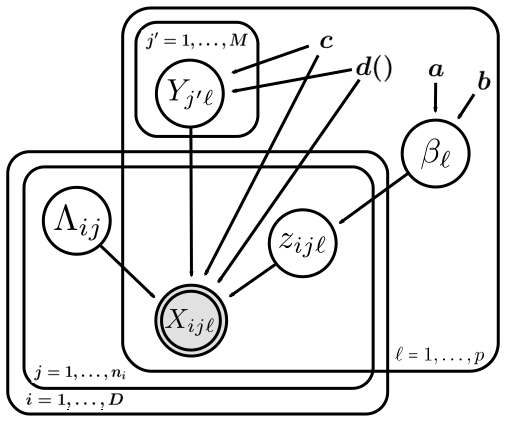
\includegraphics[width=0.35\textwidth]{figures/recordLinkage_graphicalModel}
\caption{Graphical representation of model \ref{model:string}.}
\label{fig:graphicalProcess}
\end{center}
\end{figure}

Remark: This framework was shown to work well in applications and simulation studies, however, it was quite sensitive to the choice of the hyperparameters. This method  beat supervised methods, such as random forests when the amount of training data input into the supervised methods was $< 10\%$. 

\section{Post-linkage Analysis}
There are many post-linkage analysis situations that arise in real data applications, including regression, capture recapture, networks analysis, among others. 
We present a general Bayesian approach to these, where the error can be propagated and then illustrate an example using capture recapture and networks analysis. [[We may just want to do one for ICML and then do a second one for the longer journal version]].

ATTN: Andee: can you try writing out the post-linkage approach in a general way for tomorrow and then fill in the sections for CRC and a networks approach. 

\section{Experiments} 
\label{sec:experiments}
%We assess how well each model ``fits'' XXX four sets typical of those
%arising in real-world entity resolution applications. 

Perhaps we should look at some simulated data first to fully understand 

For each data
set, we consider four statistics: (a) the number of singleton
clusters, (b) the maximum cluster size, (c) the mean cluster size, and
(d) the 90$^{\textrm{th}}$ percentile of cluster sizes. We compare
each statistic's true value to its posterior distribution according to
each of the models. For each model and data set combination, we also
consider five entity-resolution summary statistics: (a) the posterior
expected number of clusters, (b) the posterior standard error, (c) the
false negative rate, (d) the false discovery rate, and (e) the computational run time. 

[[What else might we want to look at]]. What is standard for CRC. We should report nice summary metric here too
and state why we are doing these. 
  
\looseness=-1

\subsection{Data Sets}
\label{sec:data}

We consider XXX data sets for each of the proposed methods and the evaluation metrics. 

\textbf{Restaurant:} This data set comes from XXX. There are 864 total records
and 4 fields, including XXXX. Using the unique identifiers we find that there are 
112 pairs of records that point the the same entity and there are 752 unique entities. 
Ground truth is available based upon XXX; roughly XX of the clusters are singletons. 
\looseness=-1

\textbf{CD:} This data set comes from XXX. There are 9,763 total records
and  106 fields, including XXXX. Using the unique identifiers we find that there are 
299 pairs of records that point the the same entity and there are 9,508  unique entities. 
Ground truth is available based upon XXX; roughly XX of the clusters are singletons. 
\looseness=-1

%\textbf{Voter:} This data set comes from XXX. There are 324,074 total records
%and 6 fields, including first and last name, address, telephone number, XXX. 
%Using the unique identifiers we find that there are 
%70,359 pairs of records that point the the same entity and there are 255,447 unique entities. 
%Ground truth is available based upon XXX; roughly XX of the clusters are singletons. 
%\looseness=-1

\textbf{Cora}
Add the Cora data set. 
\looseness=-1

\subsection{Results}
\label{sec:results}

We report the results of our experiments in table~\ref{tab:1} and
figure~\ref{fig:1}. 


\section{Summary}
\label{sec:disc}

\looseness=-1


\newpage

old material for paper. 
 
\vspace{-2mm}
\section{Bayesian Record Linkage}
\label{sec:background}
We assume a graphical model for record linkage that can be viewed as a hit and miss model [[CITE]], and incorporates both both categorical and noisy string data, such as names, addresses, etc. \cite{steorts15entity}. We extend this approach to a general population sized estimation framework and [[develop some other results]]. 


\subsection{Notation}
\label{sec:notation}

{Let $\bX=(X_1,\ldots,X_n)$} represent the data, with $k$ databases, indexed by~$i$.  The $i$th list has $n_i$ observed records, indexed by~$j$.  Each record corresponds to one of $N$ latent entities, indexed by $j'.$ Assume
 $N=\sum_{i=1}^k n_i$ without loss of generality.
% since there can be at most $\sum_{i=1}^k n_i$ distinct latent entities to which any record refers.
Each record or latent entity has values on $p$~fields, indexed by~$\ell$, and are assumed  be categorical and the same across all records and entities \cite{steorts14smered,steorts??bayesian}.
$M_\ell$ denotes the number of possible categorical values for the $\ell$th field.
%
In both models, $X_{ij\ell}$ denotes the
observed value of the $\ell$th field for the $j$th record in the $i$th list,
and $Y_{j'\ell}$ denotes the true value of the $\ell$th field for the $j'$th latent
entity. Then $\Lambda_{ij}$ denotes the latent entity to which the
$j$th record in the $i$th list corresponds, i.e., $X_{ij\ell}$ and $Y_{j'\ell}$
represent the same entity if and only if $\Lambda_{ij}=j'$.
%
Then $\bm\Lambda$ denotes the $\Lambda_{ij}$ collectively.
Distortion is denoted by $z_{ij\ell}=I(X_{ij\ell}\ne Y_{\Lambda_{ij}\ell})$,
where $I(\cdot)$ denotes the indicator function.
As usual,  $I$ represents the indicator function (e.g., $I(x_{ij\ell}=m)$ is 1 when
the $\ell$th field in record $j$ in file $i$ has the value $m$),
and let $\delta_a$ denote the distribution of a point mass at $a$ (e.g., $\delta_{y_{\Lambda_{ij}\ell}}$). 

\subsection{Empirical Bayesian Record Linkage}
\label{sec:string}
The work of \cite{steorts15entity} 
assumes  fields $1,\ldots,p_s$ are string-valued, while fields $p_s+1,\ldots,p_s+p_c$ are categorical, where $p_s+p_c=p$ is the total number of fields. They assume an empirical Bayesian distribution on the latent parameter. For each $\ell\in\{1,\ldots,p_s+p_c\}$, let $S_\ell$ denote the set of \emph{all} values for the $\ell$th field
that occur anywhere in the data, i.e.,
$S_\ell=\{X_{ij\ell}:1\le i\le k, 1\le j\le n_i\},$
and let $\alpha_\ell(w)$ equal the empirical frequency of value~$w$ in field~$\ell.$
%
Let $G_\ell$ denote the empirical distribution of the data in the $\ell$th field from all records in all databases combined.  So, if a random variable~$W$ has distribution $G_\ell$, then for every $w\in S_\ell$,
$P(W=w)=\alpha_\ell(w)$.
Hence, let $G_\ell$  be the prior for each latent entity $Y_{j'\ell}$. 
%
%Due to such changes in the model, the distortion process also changes to the following: 
The distortion process changes such that
\begin{align*}
%\label{model:string}
P(X_{ij\ell}&=w\mid\Lambda_{ij},Y_{\Lambda_{ij}\ell},z_{ij\ell}) \\
&=\dfrac{\alpha_\ell(w)\,\exp[-c\,d(w,Y_{\Lambda_{ij}\ell})]}{\sum_{w\in S_\ell}\alpha_\ell(w)\,\exp[-c\,d(w,Y_{\Lambda_{ij}\ell})]},
\end{align*}
where $c > 0$ is a fixed normalizing constant corresponding to an arbitary distance metric $d(\cdot,\cdot)$.  Denote this distribution by $F_\ell(Y_{\Lambda_{ij}\ell})$.
The model becomes
\begin{align}
\label{model:string}
X_{ij\ell}\mid \Lambda_{ij},\,Y_{\Lambda_{ij}\ell},\,z_{ij\ell}\;&\stackrel{\text{ind}}{\sim}\begin{cases}\delta(Y_{\Lambda_{ij}\ell})&\text{ if }z_{ij\ell}=0\\F_\ell(Y_{\Lambda_{ij}\ell})&\text{ if }z_{ij\ell}=1, \ell\le p_s\\G_\ell&\text{ if }z_{ij\ell}=1, \ell>p_s\end{cases} \notag \\
%&\qquad\text{for each }i\in\{1,\ldots,k\},\; j\in\{1,\ldots,n_i\},\; \ell\in\{1,\ldots,p_s+p_c\},\\
%&\qquad\text{with everything independent},\\
Y_{j'\ell}\;&\stackrel{\text{ind}}{\sim}G_\ell \notag \\
z_{ij\ell}\mid\beta_{i\ell}\;&\stackrel{\text{ind}}{\sim}\text{Bernoulli}(\beta_{i\ell}) \notag\\
\beta_{i\ell}\;&\stackrel{\text{ind}}{\sim}\text{Beta}(a,b) \notag \\ 
\Lambda_{ij}\;&\stackrel{\text{ind}}{\sim}\text{Uniform}\left(1,\ldots,N\right),
\end{align}
%where $i\in\{1,\ldots,k\}$, $j\in\{1,\ldots,n_i\}$, $\ell\in\{1,\ldots,p_s+p_c\}$, and $j'\in\{1,\ldots,N\}$, and
where all distributions are also independent of each other; assume that $a,b, N$ are assumed known. Finally, observe that record linkage and de-duplication are both simply a question of whether $\Lambda_{i_1,j_1}=\Lambda_{i_2,j_2}$, where $i_1\ne i_2$ for record linkage and $i_1=i_2$ for de-duplication. 


Remark: This framework was shown to work well in applications and simulation studies, however, it was quite sensitive to the choice of the hyperparameters. This method  beat supervised methods, such as random forests when the amount of training data input into the supervised methods was $< 10\%$. 

Figure~\ref{fig:graphicalProcess} contains a graphical representation of model \ref{model:string}.

\begin{figure}[htbp]
\begin{center}
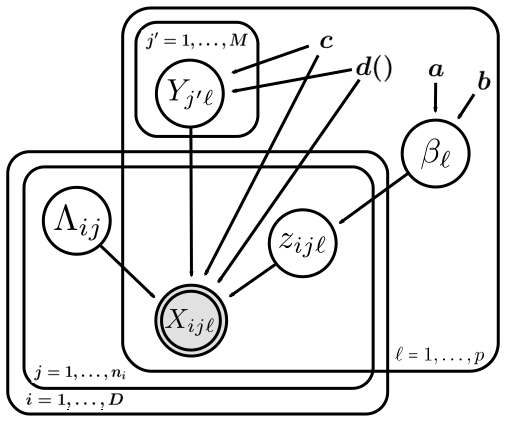
\includegraphics[width=0.35\textwidth]{figures/recordLinkage_graphicalModel}
\caption{Graphical representation of model \ref{model:string}.}
\label{fig:graphicalProcess}
\end{center}
\end{figure}

Theorem: Show that this model is a special case of the microclustering models from my NIPS paper. This is not too complicated. I just need to write out the proof. 

%\section{Blocking}
%Integrate blocking like I did in my EB paper and my previous blocking paper. Maybe write the blocking code into a package? 
%We could also ignore this since the we cannot easily propagate the errors from blocking except maybe using locality sensitive hashing because it's probabilistic. This would take more thought and could be an extension paper. 

\subsection{Record Linkage Uncertainty} 
It is most natural to quantify the uncertainty of the record linkage process, which arises from the posterior distribution of $p(\lam \mid \bX).$ 

We will assume without loss of generality that this posterior, such as the one, we have presented is a proper distribution. [[We could extend this to Gibbs models actually and these will still be proper]]. Then assuming we knew the true value of the linkage structure $\lam$, we could represent our beliefs about the population size $N$ by the posterior denoted by $p_C(N \mid n(\lam))$, which is just the posterior obtained from a capture-recapture model $C$ with some likelihood and prior distribution. Given this setup, it is most natural to account for the record linkage uncertainty in the population size by the following quantity:
\begin{align}
U(N) =: E_{\lam \mid \bX} [p_C(N \mid \n(\lam)] = \sum_{\lam} p_C(N\mid \n(\lam) p(\lam \mid \bX).
\end{align}

Remark: We can think of $U(N)$ as the expected posterior distribution of the population size, where we have averaged over the posterior of the linkage structure. In addition, it is quite easy to see that $U(N)$ is a proper distribution. Finally, the total variability represented by $U(N)$ can also be easily decomposed. 

Recall $U(N) = p(N \mid \bX).$ Then 
\begin{align}
\Var (N\mid X) = \Var_{\lam \mid \bX} [E[N \mid \lam ]] + E_{\lam \mid \bX} [\Var[N \mid \lam ]],
\end{align}
where
$\Var_{\lam \mid \bX} [E[N \mid \lam ]]$
corresponds to record linkage uncertainty due to population size estimation and 
$E_{\lam \mid \bX} [\Var[N \mid \lam ]]$
correspond to the variability associated from a Bayesian methods due to estimating $N.$ (In practice, both $U(N)$ and both quantities above must be estimated by Markov chain Monte carlo).


\section{Population Size Estimation}
%Introduce the idea of capture recapture. Try using some ideas from Madigan and York and then try extending this to more realistic scenarios. 
We first introduce a general framework for inclusion pattens for population sized estimation. Next, we derive a way of measuring the record linkage uncertainty of Bayesian graphical models. In addition, we look at a general way the variability for record linkage and capture recapture can be assessed. Finally, we work out this formulation under the framework of Madigan and York (1992) and [[let's try and go for that of Johndrow and Valllier]]. 

\subsection{Capture Recapture Inclusion Patterns} 
Let $\h =(h_1,\ldots,h_K) \in \{0,1\}^K$ denote the inclusion pattern, where $h_k=1$ indicates inclusion in database $k.$ Let $n_{\h}$ denote the number of entities with inclusion pattern $\h,$ where the inclusion pattern's frequencies are in a contingency table $n^* = \{n_{\h} \}$ where $\h \in \{0,1\}^K.$ Of course, the number of entities missed by all databases is unobserved and missing, $n_{00\cdots}$, and thus, the observed counts are denoted by $\{n_{\h} \}$ where $\h \in \{0,1\} \setminus \{0\}^K.$

For a particular entity, their inclusion pattern $\h$ can be written such that $Pr(\h \mid \boeta) = \boeta_{\h}$, where $\boeta = (\eta_1, \cdots, \eta_K)$ gives the probability of each inclusion pattern. Each model will dictate different inclusion patterns; let $\boeta_m$ denote the inclusion probabilities under model $m.$ Assuming $N = \sum_{\h} n_{h}$ entities in the population and assuming that each entity is indendently and identically distributed, we find that 
\begin{align}
P(\n^{*} \mid N, \boeta_m, m) = N! \prod_{\h \in \{0,1\}} 
\frac{
(\boeta_{\h,m})^{n_{\h}}}
{n_{\h}!}
\end{align}

Since in practice $N$ and $\n$ are fixed, we can write $n_{00\cdots0} = N - \sum_{\h \in  \{0,1\}^K \setminus \{0\}^K} n_{h}$. It then follows that 
$P(\n \mid N, \boeta_m, m) = P(\n^{*} \mid N, \boeta_m, m).$ Now given any model $m$ and a prior on the population size p(N), our main goal is to obtain

\begin{align}
P(N \mid \n, m) = \frac{
P(\n \mid N, m) p(N)
}
{
\sum_N P(\n \mid N, m) p(N),
}
\end{align}
where 
$
P(\n \mid N, m) = \int_{\boeta_m} 
P(\n \mid N, \boeta_m, m) p(\boeta_m \mid m) \; d \boeta_m.
$

The above formulation only requires that $N$ and $\boeta_m$ are independent. We could consider model that should lead to a closed form solution such as those in Madigan and York \url{https://pdfs.semanticscholar.org/7aed/b2eb2345c1d6ef844be7a58bcca3f7f9cb78.pdf}, or perhaps \url{https://arxiv.org/pdf/1606.02235.pdf}. 

The Madigan and York paper is super cool because it allows us to do Bayesian model averaging, so we could write out the Bayesian partition models and average over all of the priors that we might believe in and then incorporate the record linkage error. 

Recall that our modeling framework can be viewed as a bi-partite graph, which has strong connections to probabilistic graphical models [[CITE]], where in this literature one encodes the set of conditional independencies of a multivariate distribution into a graph using edges and nodes. In a graphical model (and in our framework), a node is represented by a random variable, and two nodes are joined if they are conditionally dependent given all the other nodes or random variables. Thus, a graphical model captures conditional dependencies between two nodes of inclusion patterns intrinsically. Madigan and York (1992, 1997) restrict to working with decomposable graphical models, meaning that the independence graph is triangulated (chordal). One reason we prefer to work with this approach is that the conditionals are available in closed form and we show the details of this below.

Given a model $m$ and a set a parameters $\boeta_m$, we can use the hyper-Dirichlet distribution (Dawid and Lauritzen, 1993 and Madigan and York (1992) for the parameters $\boeta_m$, which lead to a closed form solution for $P(\n \mid N,m).$ (We refer to Dawid and Lauritzen, 1993 regarding a review of the hyper-Dirchlet distribution). Thus, given a hyper-Dirichlet prior on $\boeta_m$ and assuming that $N$ and $\boeta_m$ are independent, Madigan and York (1992) show that 
\begin{align}
P(\n \mid N, m) &= \int_{\boeta_m} 
P(\n \mid N, \boeta_m, m) p(\boeta_m \mid m) \; d \boeta_m \\
&= 
\frac{N!}
{\prod_{\h \in  \{0,1\}^K} n_{\h}! }
\frac{\Phi_m(\balpha + \n^{*})}
{\Phi_m(\balpha)}
\end{align}.

Note that
\begin{align}
\Phi_m(\balpha)
&=
\frac{
\prod_{\ell=1}^L 
\prod_{\h_{ C{\ell} }}
\Gamma(\alpha_{\h_{C_{\ell}}})
}
{
\Gamma(\sum_{\h \in \{0,1\}^K} \alpha_{\h})^Q
\prod_{\ell=2}^L 
\prod_{\h_{ S{\ell} }}
\Gamma(\alpha_{\h_{S_{\ell}}})
}
\end{align}
where
$\{C_\ell\}$ denotes the set of maximal cliques, $\{S_\ell\}$ the set of separators, and $Q$ the set of connected components. In addition, for a subset of nodes $O$, $\h_O$ represents an inclusion pattern constrained to the subset of variables in $O.$ Also, 
$$\alpha_{\h_O} = \sum_{\h^{\prime}: \h_{O}^{\prime} = \h_O} \alpha_{\h^{\prime}}.$$
Within this framework, it is natural to take into account the uncertainty regarding the population sized estimation, which can be written as 

$$P(N \mid n)  = \frac{ P(N) \sum_m P(\n \mid N, m) p(m)  }
{\sum_N P(N) \sum_m P(\n \mid N, m) p(m)} $$
for prior distributions $p(m).$ 

(Perhaps we want to look at uniform priors to start and adjust from there). 

\section{Population Sized Estimation Post Record Linkage}

\textcolor{red}{We should be able to write this down as mixture models using BNP.} 
Given a linkage structure, we first describe how to compute the contingency table (incomplete) $\n.$ Let $n$ denote the total number of labelings that occur in the linkage structure $\lam.$ Without loss of generality, we can write the labelings of $\lam$ as being $1,\ldots,n.$ Then for each label
$\lambda = 1,\ldots,n$ let 

$$
H_{\lambda,k} =
\begin{cases}
1, \text{ if there exists a record $(i,j) \in \bX$ such that $\lambda_{i,j} = \lambda$} \\
0, \text{otherwise}. \\
\end{cases}
$$

That is, $H_{\lambda,k}$ contains inclusion indicators of where each of the $n$ individuals are included in database $k$, and then we obtain the $\n(\lam)$ contingency table using these inclusion indicators. Note that we write $\n(\lam)$ since each contingency table is a function of the linkage structure.



\subsection{Details under particular models, like Madigan and York, Johndrow and Vallier} 
Sketch out the details next for Madigan and York.
Then do so for the Johndrow paper. 

\section{Things to look at next}

Now, all we need to do is write down how to perform this in practice and how to evaluate the uncertainty. We also need to try this out in practice. 
It might be interesting to look at graphs that aren't decomposable or see if the framework of Johndrow and Manrique-Vallier fits in at all. 

It seems that we could work with a very large class of capture-recapture models, starting with a stick-breaking process, a MFM, a DPM, and potentially others. The record linkage model can be viewed at some level as a stick breaking process. 

\begin{enumerate}
\item The Madigan and York model will be limiting but in closed form. 
\item I think we can also write all the Kolchin partition models down in closed form as well. We can at least start with the approach of Johndrow and
Vallier, but special cases that follow are a DP, PYP, NBD, NBNB. This would be quite nice. Could the Madigan and York be a special case of a KP model? This would be quite interesting. 
\item It would be nice to tie some of this together because it would make a very general framework.
\end{enumerate}


\section{Issues with the approach}

[[There is an issue with Madigan and York as they require that models be decomposable or rather that the graph be a triangle. We want graphs to be able to have any type of form, so this is a weakness of their proposal]].

This deals with graphs that should be able to be non-decomposable \url{http://citeseerx.ist.psu.edu/viewdoc/download?doi=10.1.1.440.1333&rep=rep1&type=pdf}

\section{Small Area Estmation}

A small area estimation model can be written as

$$y = \theta + X\beta + u + e$$
where the error terms are independent and Gaussian. 
Again, this is a mixture model. If you think about the approach to SAE and CRC, 
we can view them both as mixture models. We should try and write the formulation very general. 

\section{Networks}

Notes regarding the network problem. 

Think for example you want to reconstruct a relational network among some actors (may be countries, or famous people) using news media reports.  I.e. anytime some news media comes out with a news report involving say actor A and actor B you add an edge among them. Now, as we know news media reports are very noisy and computer systems processing them have additional noise. This creates lots of duplication problems in two directions:

1] Duplication in the nodes: For example two media reports may refer to the same actor, but the way the report is written may lead you to think they are two different nodes. Of course in this case record linkage will be important to solve these duplication problems in the two nodes. I.e. your network is indeed much smaller (in terms of real actors) than it seems, because sometimes you are adding nodes that indeed refer to the same actor.
2] Duplication in the edges:  Suppose news media 1 said that A and B had a conflict, whereas in the same day news media 2 said that A and B had a fight. This refers of course to the same relation (the only difference is that news media 1 used term ?conflict? and news media 1 used term ?fight?). So you should add only 1 edge instead of 2 among actors A and B. These duplications in the edges are quite common and an issue, since you end up over-counting the relations among actors.

I think you can easily find these issues in this dataset: https://www.gdeltproject.org/data.html. But I can think about many other examples in citation networks, and also brain networks (especially on the edge duplication and also nodes one when you go to voxels).

I tried to address those in  https://www.gdeltproject.org/data.html with some ad-hoc choice when I was using these data some years ago. It worked well, but I am sure that your methods here would do a great job. This is quite important in networks, since such pre-processing can provide more high-quality relational data.

One quick idea from my email exchange with Dany:

Build up the network using the raw data (without record-linkage on nodes and edges)?call it network X1? and the build up another network using data that have been de-duplicated (both nodes and edges) ? call it network X2, and then check how different the two networks are. 

I expect that:

1] They will be quite different
2] The ?cleaned? network X2, will have a structure that better fits social processes (i.e. has better communities, has small world structure etc?).

Applying your methods to these data shouldn?t be hard. Indeed, each row in your dataset is a different news media report for which you have many informations (actors, time of publication, type of news, text data,). So your record linkage problem will have news media reports as statistical units (instead of people). If you can solve the duplication problem for the news reports, then you are jointly solving both the node and edge duplication issue. In fact, you will end up with a set of unique news (in terms of actors and type of relation among them).

\newpage

Notes for paper. Cannot get our PSD paper to compile. 

AK: We'll want to talk about notation here. 

It can be shown that a special case of [[CITE]] is equivalent to the linkage structure
prior~\cite{steorts14smered,steorts??bayesian}, which we now explicitly formalize. 
We review the model of [[CITE]] in the special case and then show the equivalence of 
the models. 

Let K be the number of potential clusters. Then following [[CITE]], we have the following 
model: 
\begin{align}
  K &\sim \textrm{NegBin}\,(a, q) \nonumber \\
 N_1, \ldots, N_K &\g K \iid \textrm{NegBin}\,(r, p),
  \label{eqn:nbnb}
\end{align}
for $a, r \,>\, 0$ and $q, p \in (0, 1)$. Note that $K$ and some of
$N_1, \ldots, N_K$ may be zero. We then define $N = \sum_{k=1}^K N_k$
and, given $N_1, \ldots, N_K$, generate a set of cluster assignments
$z_1, \ldots, z_N$ by drawing a vector uniformly at random from the
set of permutations of $$(\underbrace{1,\ldots,1}_\text{$N_1$
  times},\underbrace{2,\ldots,2}_\text{$N_2$
  times},\ldots\ldots,\underbrace{K,\ldots,K}_\text{$N_K$ times}).$$

The cluster assignments $z_1, \ldots, z_N$ induce a random partition
$C_N$ of $[N]$, where $N$ is itself a random variable---i.e., $C_N$ is
a random partition of a random number of elements. The resulting marginal distribution of $C_N$ the NegBin--NegBin (NBNB)
model. If $\mathscr{C}_N$ denotes the set of all possible partitions
of $[N]$, then $\bigcup_{N=1}^{\infty} \mathscr{C}_N$ is the set of
all possible partitions of $[N]$ for $N \in \mathbb{N}$. If one replaces the 
 negative binomials in equation~\ref{eqn:nbnb} with Poissons, then
we obtain a limiting special case of the NBNB model. We will refer to this
model the permuted Poisson sizes (PERPS) model.

We now show the equivalence of the model of PERPS to that in equation \ref{}. 
Let $Z = (z_1, \ldots, z_n).$
According to the model defined by PERPS$(\alpha,\lambda),$ 
\begin{equation}
  P(Z \g K) = P(Z, N \g K) = P(Z \g N, K)\,P(N \g K)
  \end{equation}
since the value of $N$ is completely determined by the value of
$Z$. From the Poisson superposition principle, we know that if $N =
\sum_{k=1}^K N_k$ and $N_1, \ldots, N_K \g K \iid \Poisson(\lambda)$,
then $N \g K \sim \Poisson(K \lambda)$ and
\begin{equation}
  P(N \g K) = \frac{(K \lambda)^N}{N!} \exp{(-K \lambda)}.
  \end{equation}
We also know that $P(Z \g N, K) =
\left(\frac{1}{K}\right)^N$. Therefore,
\begin{equation}
  \label{eqn:prob_z_given_k}
  P(Z \g K) = \frac{\lambda^N}{N!} \exp{(-K \lambda)}.
  \end{equation}
We show that
equation~\ref{eqn:prob_z_given_k} holds by writing $P(Z \g K)
= P(Z, N, S_1, \ldots, S_K \g K)$ since $N$ and $S_1, \ldots, S_K$ are
completely determined by $Z$. It then follows that
\begin{align}
  &P(Z \g K) \\ &= P(Z, N, S_1, \ldots, S_K \g K)\\
  &= P(Z \g N, S_1, \ldots, S_K, K) \, P(N, S_1, \ldots, S_K \g K)\\
  &= P(Z \g S_1, \ldots, S_K, K)\, P(N \g S_1, \ldots, S_K, K) \, \\
  &\qquad \times
  P(S_1, \ldots, S_K \g K)\\
  &= \frac{\prod_{k=1}^K S_k!}{N!} \cdot 1 \cdot
  \frac{\lambda^N}{\prod_k=1 S_k!} \exp{(-K \lambda)}\\
  &= \frac{\lambda^N}{N!} \exp{(-K \lambda)}.
  \end{align}
Thus, conditioning on $N,$ or rather 
$P(Z \g N, K) = \left(\frac{1}{K}\right)^N$
leads exactly \cite{steorts??bayesian,steorts14smered} to the uniform prior on the linkage structure, which clusters records to unknown latent entities in the framework of \cite{steorts??bayesian,steorts14smered}, where $N, K$ are both fixed.
%Then $$P(Z\mid K) = P(Z \mid N,K) P(N\mid K) = e^{-k \lambda} \frac{(k \lambda)^n}{n!} \times 1/k^n.$$

\emph{Remark}: Due to this, $P(Z \mid K)$ is the same for \cite{steorts??bayesian,steorts14smered} and PERPS and  it follows that $P(K)$ is the same for the PERPS and Poisson-Uniform.  This means that $P(Z)$ is the same since $P(Z\mid K)$ and $P(K)$ are the same for both models. This implies that $P(C_N \mid N)$ will be the same under our proposed framework and that of \cite{steorts??bayesian,steorts14smered}.



\clearpage
\newpage

\bibliographystyle{plain}
\bibliography{references}

\clearpage
\newpage

\appendix

%\section*{Supplementary Material}
%\label{sec:appendix}

\end{document}